\begin{figure}[h] 
\centering 
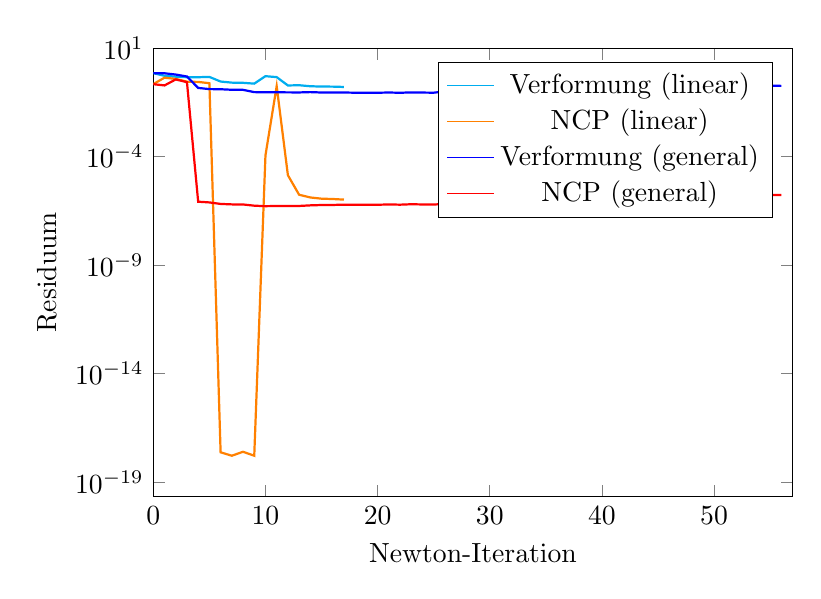
\begin{tikzpicture}[every plot/.append style={thick}] 
\begin{axis}[ 
label style={font=\normalsize}, 
xlabel={Newton-Iteration}, 
ylabel={Residuum}, 
xmin=0, xmax=57, 
ymode=log, 
ymin=0, ymax=10, 
width=0.8\textwidth, 
height=0.6\textwidth, 
legend pos=north east, 
legend style={cells={align=left}}, 
grid style=dashed, 
] 
\addplot[ 
color=cyan, 
] 
coordinates { 
(0, 7.05e-01)(1, 5.33e-01)(2, 4.86e-01)(3, 4.59e-01)(4, 4.59e-01)(5, 4.73e-01)(6, 2.90e-01)(7, 2.58e-01)(8, 2.53e-01)(9, 2.32e-01)(10, 5.12e-01)(11, 4.63e-01)(12, 1.91e-01)(13, 1.96e-01)(14, 1.76e-01)(15, 1.70e-01)(16, 1.69e-01)(17, 1.63e-01)}; 
\addlegendentry{Verformung (linear)} 
\addplot[ 
color=orange, 
] 
coordinates { 
(0, 2.21e-01)(1, 4.37e-01)(2, 3.82e-01)(3, 2.87e-01)(4, 2.78e-01)(5, 2.43e-01)(6, 2.39e-18)(7, 1.66e-18)(8, 2.53e-18)(9, 1.66e-18)(10, 1.15e-04)(11, 1.78e-01)(12, 1.40e-05)(13, 1.76e-06)(14, 1.32e-06)(15, 1.16e-06)(16, 1.12e-06)(17, 1.05e-06)}; 
\addlegendentry{NCP (linear)} 
\addplot[ 
color=blue, 
] 
coordinates { 
(0, 7.08e-01)(1, 6.96e-01)(2, 6.08e-01)(3, 4.94e-01)(4, 1.47e-01)(5, 1.30e-01)(6, 1.28e-01)(7, 1.21e-01)(8, 1.20e-01)(9, 9.42e-02)(10, 9.31e-02)(11, 9.25e-02)(12, 9.18e-02)(13, 9.12e-02)(14, 9.44e-02)(15, 9.05e-02)(16, 9.02e-02)(17, 9.04e-02)(18, 8.86e-02)(19, 8.92e-02)(20, 8.84e-02)(21, 9.03e-02)(22, 8.82e-02)(23, 9.13e-02)(24, 8.99e-02)(25, 8.87e-02)(26, 1.02e-01)(27, 1.93e-01)(28, 1.83e-01)(29, 1.83e-01)(30, 1.80e-01)(31, 1.79e-01)(32, 1.78e-01)(33, 2.00e-01)(34, 1.54e-01)(35, 1.40e-01)(36, 1.37e-01)(37, 1.41e-01)(38, 1.40e-01)(39, 1.12e-01)(40, 1.06e-01)(41, 1.16e-01)(42, 1.08e-01)(43, 1.07e-01)(44, 1.05e-01)(45, 3.56e-01)(46, 3.44e-01)(47, 3.31e-01)(48, 2.90e-01)(49, 2.86e-01)(50, 2.08e-01)(51, 1.83e-01)(52, 1.81e-01)(53, 1.80e-01)(54, 1.79e-01)(55, 1.86e-01)(56, 1.83e-01)}; 
\addlegendentry{Verformung (general)} 
\addplot[ 
color=red, 
] 
coordinates { 
(0, 2.19e-01)(1, 1.92e-01)(2, 3.62e-01)(3, 2.71e-01)(4, 8.42e-07)(5, 7.80e-07)(6, 6.65e-07)(7, 6.33e-07)(8, 6.28e-07)(9, 5.52e-07)(10, 5.24e-07)(11, 5.33e-07)(12, 5.35e-07)(13, 5.36e-07)(14, 5.71e-07)(15, 5.92e-07)(16, 5.96e-07)(17, 6.16e-07)(18, 6.05e-07)(19, 6.14e-07)(20, 6.09e-07)(21, 6.29e-07)(22, 6.14e-07)(23, 6.43e-07)(24, 6.29e-07)(25, 6.24e-07)(26, 6.63e-07)(27, 8.49e-07)(28, 7.52e-07)(29, 7.19e-07)(30, 7.23e-07)(31, 7.70e-07)(32, 7.87e-07)(33, 1.01e-06)(34, 1.09e-06)(35, 9.44e-07)(36, 9.32e-07)(37, 9.26e-07)(38, 9.51e-07)(39, 7.82e-07)(40, 7.84e-07)(41, 8.60e-07)(42, 7.76e-07)(43, 7.68e-07)(44, 6.60e-07)(45, 3.48e-06)(46, 3.35e-06)(47, 3.45e-06)(48, 2.73e-06)(49, 2.73e-06)(50, 1.87e-06)(51, 1.64e-06)(52, 1.63e-06)(53, 1.63e-06)(54, 1.63e-06)(55, 1.70e-06)(56, 1.70e-06)}; 
\addlegendentry{NCP (general)} 
\end{axis} 
\end{tikzpicture} 
\caption{Residuen des Stoffgesetzes 'St.Venant' mit Hinderniss 'Parabel' und 2178 Freiheitsgraden für die Verschiebung.} 
\label{fiq:St.Venant_Parabel_level4} 
\end{figure} 
